\documentclass{llncs}
\usepackage{graphicx}     
\usepackage{cite}
\usepackage{amssymb,amsmath}
\usepackage{algorithm}
\usepackage[noend]{algorithmic}
\usepackage{array}
\usepackage{color}
%\usepackage{hyperref}

\newcommand{\Acronym}[1]{\ensuremath{{\small{\texttt{#1}}}}}
\newcommand{\Symbol}[1]{\ensuremath{\mathcal{#1}}}
\newcommand{\Function}[1]{\ensuremath{{\small \textsc{#1}}}}
\newcommand{\Constant}[1]{\ensuremath{\small{\texttt{#1}}}}
\newcommand{\Var}[1]{\ensuremath{{\small{\textsl{#1}}}}}
\newcommand{\False}{\Constant{false}}
\newcommand{\True}{\Constant{true}}
\newcommand{\Null}{\Constant{null}}
\newcommand{\Name}{\Acronym{Name}}
\newcommand{\Revision}[1]{\textcolor{red}{#1}}
\newcommand{\R}{\ensuremath{\mathbb{R}}}
\newcommand{\Traj}{\ensuremath{\zeta}}
\newcommand{\Tree}{\Symbol{T}}
\newcommand{\LTLNext}{\bigcirc}
\newcommand{\LTLEventually}{\Diamond}
\newcommand{\LTLAlways}{\Box}
\newcommand{\LTLUntil}{\cup}
\newcommand{\LTLRelease}{\Symbol{R}}
\newcommand{\Automaton}{\Symbol{A}}


 \begin{document}

\frontmatter
\pagestyle{headings}  
\addtocmark{} 

\mainmatter 

\title{Motion Planning for Swarms by Combining Probabilistic Roadmaps and
  Potential Fields}

\author{Alex Wallar\inst{1} \and Erion Plaku\inst{2}}

\institute{
Department/School name, University, Address
\and
Dept. of Electrical Engineering and Computer Science\\ 
Catholic University of America, Washington DC 20064 USA
}


\maketitle
\begin{abstract}
This paper combines probabilistic roadmaps with potential fields in
order to enable a swarm of boids to effectively move to a desired
destination while avoiding collisions with obstacles and each
other. Potential fields provide the boids with local, reactive,
behaviors that seek to keep the swarm moving together and away from
the obstacles. The probabilistic roadmap provides global path planning
which guides the swarm through a series of intermediate goals in order
to effectively reach the desired destination. Random walks in
combination with adjustments to the potential fields and intermediate
goals are used to help stuck boids escape local minima.  Experimental
results provide promising validation on the efficiency
and scalability of the proposed approach.
\end{abstract}


\section{Introduction}
\label{sec:Intro}

\section{Method}
\label{sec:Method}

$\Name$ combines probabilistic roadmaps with potential fields in order
to enable a swarm of boids to effectively move to a desired
destination while avoiding collisions with obstacles and each other.
The probabilistic roadmap provides global path planning to determine
appropriate intermediate goals for the swarm. The potential
fields provide local planning to enable the boids move together as a swarm
towards the goal while avoiding collisions. More specifically, the swarm
motions are governed by the following criteria:
\begin{enumerate}
\item Boids are repulsed from obstacles.
\item Boids move as a swarm while keeping some separation from one another.
\item A boid's heading is influenced by the headings of its neighbors.
\item There is long range attraction to intermediate goals and final destination. 
\end{enumerate}
To avoid collisions with obstacles, $\Name$ creates a strong repulsive potential
field, denoted as $PF_\Var{obst}(b)$, which
pushes each boid $b$ away from the obstacles. The repulsive potential
increases quadratically with respect to the inverse of the distance
from the boid to the obstacles. Such rapid increase prevents the boids
from getting too close to the obstacles. 

To maintain separation among the boids in the swarm, each boid is
pushed away from its neighbors. A weak sigmoidal repulsive
potential, denoted as $PF_\Var{boids}(b)$, is employed rather than a
strong quadratic repulsive potential in order to push $b$ away
from its neighbors but not so strongly as to separate it from the
swarm.

To move as a swarm, a boid's heading is influenced by the headings of
its neighbors, defined as $PF_\Var{heading}(b)$. To promote effective
movements, preference is given to neighbors that are not
stuck and are neither too close nor too far. The headings of the
neighbors that are chosen are averaged and combined with the other
potential fields to determine the new heading and position of each
boid.



\begin{algorithm}[t]
\caption{Pseudocode for $\Name$}
\label{algo:Main}
\begin{algorithmic}[1]
\setcounter{ALC@line}{0}
%\COMMENT{generate $n$ additional roadmap vertices}
\vspace*{1mm}
\STATE $RM = (V, E) \leftarrow \Function{ConstructRoadmap}()$, where
\STATE \hspace*{5mm} $V \leftarrow$ sample numerous random points, discard those that are in collision 
\STATE \hspace*{5mm} $E \leftarrow$ connect neighboring points in $V$,
discard those edges that are in collision
\STATE \hspace*{5mm} $w(q_i) \leftarrow$ assign weight to each vertex $q_i \in V$
\STATE \hspace*{5mm} $w(q_i, q_j) \leftarrow$ assign weight to each edge $(q_i, q_j) \in E$
\STATE $\zeta = [q_k]_{k=1}^m \leftarrow
\Function{IntermediateGoals}(RM)$ \hfill{\emph{$\diamondsuit$ obtained from shortest path}}
\STATE $\Var{igoal}(b) \leftarrow \zeta(1)$
\hfill{\emph{$\diamondsuit$ set current intermediate goal for each
    boid}}

\WHILE{$\Function{solved}() = \False$}
\FOR{$b \in \Var{Boids}$ with $\Function{ReachedIntermediateGoal}(b) =\True$} 
\STATE $\Var{igoal}(b) \leftarrow \Function{NextIntermediateGoal}(\zeta)$
\ENDFOR

\FOR{$b \in \Var{Boids}$ }
\STATE $PF(b) \leftarrow \Function{superimpose}(PF_\Var{obst}(b),
PF_\Var{boids}(b), PF_\Var{igoal}(b), PF_\Var{heading}(b), PF_\Var{escape}(b))$
\STATE $\Var{NewHeading}(b) \leftarrow w_1 \Var{heading}(b) + w_2 PF(b)$
\ENDFOR

\FOR{$b \in \Var{Boids}$ }
\STATE $\Var{heading}(b) \leftarrow \Var{NewHeading}(b)$; $\quad$ 
$\Var{pos}(b) \leftarrow \Var{pos}(b) + \Var{heading}(b)$
\ENDFOR
\ENDWHILE


\end{algorithmic}
\end{algorithm}



To guide the swarm towards the final destination, global path planning
based on probabilistic roadmaps is used to determine suitable
intermediate goals. A probabilistic roadmap is constructed by sampling
collision-free points and connecting neighboring points with
collision-free edges to obtain a graph that captures the connectivity
of the environment. Roadmap vertices and edges are associated with
weights that estimate the feasibility of the swarm to pass through
their surrounding areas. The shortest path in the roadmap to the final
destination is used to provide a series of intermediate goals that the
swarm can follow to effectively reach the final destination. An
attractive potential, denoted as $PF_\Var{igoal}(b)$, is added between
each boid $b$ and its current intermediate goal. When the boid reaches the
current intermediate goal, the next point in the shortest path is set
as the new intermediate goal.

The different potential fields are superimposed to obtain the overall
force vector applied to each boid $b$. In this way, the potential
field on the boid $b$ exerts a strong repulsive potential away from
the obstacles while attracting it to the current intermediate goal,
maintaining a separation distance from the other boids, and adjusting
the heading so that the boids move as a swarm toward the final
destination. If a boid gets stuck in local minima, random walks in
combination with adjustments to the potential fields and intermediate
goals are used to help it escape.  Pseudocode for the
overall approach is given in Algo.~\ref{algo:Main}. Details of the
main steps follow.

\subsection{Roadmap Construction}
\label{sec:RM}

Drawing from PRM \cite{PRM} approaches, $\Name$ constructs a roadmap
in order to effectively guide the swarm toward the goal. Since the
swarm could have many robots, the roadmap is not constructed over the
entire high-dimensional configuration space, as it is often the case
in PRM approaches, but is instead constructed over the low-dimensional
workspace where the swarm moves. As explained in this section, $\Name$
uses the roadmap to find intermediate areas in which the swarm can
move to effectively reach the goal.

\subsubsection{Roadmap Vertices:}
The roadmap is constructed by first sampling a large number of points
uniformly at random inside the workspace boundaries and then
discarding all the points that are in collision or too close to an
obstacle. A parameter, $d_\Var{clear}$, determines the minimum
acceptable distance from a sampled point to the nearest obstacle. The
remaining points, which are all at least $d_\Var{clear}$ units away
from the obstacles, are added as vertices to the roadmap graph $RM =
(V, E)$. A roadmap vertex $q_i$ and the clearance $d_\Var{clear}$
conceptually define a clearance area as a disk centered at $q_i$ with
radius $d_\Var{clear}$, denoted as $\Var{area}(q_i)$. In order to bias
the swarm movements toward less cluttered areas, each roadmap vertex
$q_i$ is associated with a weight $w(q_i)$ which estimates how
feasible it is for the swarm to travel through $\Var{area}(q_i)$. More
specifically, the weight is defined as
$$
w(q_i) = \left(\sum_{o \in \Var{Obstacles}} \Var{dist}(q_i, o)\right)^3,
$$ where $\Var{dist}(q_i, o)$ denotes the minimum distance from $q_i$
to the obstacle $o$. In this way, small weights indicate the presence
of obstacles nearby, which may make it more difficult for the swarm to
pass through.  As explained later in the section, $\Name$ gives
preferences to roadmap vertices associated with high weights which are
indicative of areas with high clearance. Note that other definitions
for the weight function are possible. The particular function used in
this paper worked well for the experiments as it captures the desired
properties of biasing the swarm movements towards less cluttered
areas.

\subsubsection{Roadmap Edges:}
After generating roadmap vertices, $\Name$ connects each
roadmap vertex to its $k$ nearest neighbors. Edges that are in
collision are discarded. The weight of an edge connecting $q_i$ to
$q_j$ is defined as
$$
w(q_i, q_j) = ||q_i, q_j||_2 / \min(w(q_i), w(q_j)),
$$
where $||q_i, q_j||_2$ is the Euclidean distance from $q_i$ to $q_j$. Note
that $w(q_i, q_j)$ is small when $q_i$ and $q_j$ are close to each
other and away from obstacles.

%$s_\Var{edge}$ is a scaling constant to account for the workspace dimensions and

\subsubsection{Intermediate Goals along Shortest Roadmap Path:} Dijkstra's shortest-path
algorithm is used to compute the shortest path $\zeta$ in the roadmap
to the final destination, where the weight of a roadmap edge $(q_i, q_j)$ is
defined by $w(q_i, q_j)$ as described above. Each vertex $q_k \in
\zeta$ defines an intermediate goal for the swarm. More specifically,
$\Name$ seeks to move the swarm to the goal by passing through the
areas $\Var{area}(q_k)$ as defined by the vertices $q_k$ along the
shortest path $\zeta$. Note that the dependency of the edge weights
on vertex weights ensures that the shortest path in the roadmap does
not come too close to the obstacles, which could lead the swarm to
often get stuck in local minima.

\subsection{Potential Fields}
\label{sec:PF}

\subsubsection{Repulsion from Obstacles:}
\label{sec:PFobst} An imperative objective for
the swarm is to always avoid collisions with obstacles. For this
reason, a repulsive potential is defined that pushes the boids away
from the obstacles. More specifically, the repulsive potential between
a boid $b$ and an obstacle $o$ is defined as
$$ P_\Var{obst}(b, o) = \frac{1}{(\Var{dist}(\Var{pos}(b), o) - \Var{radius}(b))^2},
$$ where $\Var{pos}(b)$ and
$\Var{radius}(b)$ denote the position and radius of the boid $b$, respectively. Note that the
important aspect of this repulsive function is that its value
increases rapidly as the boid approaches an obstacle. This ensures
that the boid would be pushed away and never collide with an obstacle.

%$$ P_\Var{obst}(b, o) = \frac{s_\Var{obst}\,
%  \Var{radius}(b)}{(\Var{dist}(\Var{pos}(b), o) - \Var{radius}(b))^2},
%$$ where $s_\Var{obst}$ denotes a scaling constant and $\Var{pos}(b),
%\Var{radius}(b)$ denote the boid position and radius. Note that the
%important aspect of this repulsive function is that its value
%increases rapidly as the boid approaches an obstacle. This ensures
%that the boid would be pushed away and never collide with an obstacle.

In order to limit the influence of the obstacles that are far away,
the repulsion is computed only from those obstacles that are within a
certain distance $\Delta_\Var{obst}$ from the boid. The potential
field imposed by the obstacles is then defined as 
$$
PF_\Var{obst}(b) = \sum_{\stackrel{o \in
    \Var{Obstacles}}{\Var{dist}(b, o) \leq \Delta_\Var{obst}}} (\Var{pos}(b)
- \Var{ClosestPoint}(o, \Var{pos}(b))) P_\Var{obst}(b, o),
$$
where $\Var{ClosestPoint}(\Var{pos}(b), o)$ denotes the closest point on the
obstacle $o$ to $\Var{pos}(b)$.

\subsubsection{Repulsion from other Boids:}
\label{sec:PFboids} As the swarm moves,
the boids need to avoid coming too close to each other as it
could lead to collisions. At the same time, the boids should not be
far away from each other in order to move as a swarm. To achieve these
objectives, $\Name$ uses a weak repulsive sigmoid function
$$
P_\Var{boids}(b_i, b_j) = \frac{1}{1 +
  \exp(\delta_\Var{boids}\, ||\Var{pos}(b_i), \Var{pos}(b_j)||_2)},
$$
where $\delta_\Var{boids}$ is a scaling constant.
In order to limit the influence of the boids that are far away,
similar to the potential field for obstacles,
the repulsion is computed only from those boids that are within a
certain distance $\Delta_\Var{boids}$. The potential
field imposed on the boid $b$ by the other boids is then defined as 
$$
PF_\Var{boids}(b) = \sum_{\stackrel{b_i \in
    \Var{Boids} - \{b\}}{\Var{dist}(b, b_i) \leq \Delta_\Var{boids}}} (\Var{pos}(b)
- \Var{pos}(b_i)) P_\Var{boids}(b, b_i).
$$
In this way, the boids travel close together but are
pushed away when the come too close to one another.

\subsubsection{Attraction to the Current Intermediate Goal:}
\label{sec:PFigoal} As
discussed, $\Name$ uses the shortest path $\zeta$ in the roadmap to
set the intermediate goals for the swarm. Let $\Var{igoal}(b)$ denote
the current intermediate goal of the boid $b$. Note that
$\Var{igoal}(b)$ is associated with some point $q_k$ in $\zeta$. An
attractive potential field that
pulls the boid $b$ towards $\Var{igoal}(b)$ is then defined as 
$$
PF_\Var{igoal}(b) = \frac{\Var{igoal}(b) - \Var{pos}(b)}{1 +
  \exp(\delta_\Var{igoal}\, ||\Var{pos}(b), \Var{igoal}(b)||_2)},
$$ where $\delta_\Var{igoal}$ is a scaling constant. Although other
definitions are possible, the sigmoid function allows the boids to
reach the goal without getting too greedy, which could lead to getting
stuck in local minima. When $b$ reaches $\Var{igoal}(b)$, the next
point $q_{k+1}$ in the shortest path $\zeta$ is set as the new
intermediate goal for $b$.

\subsubsection{Influence of Neighbors on Heading:}
\label{sec:PFheading}
 In order to make
the boids move as a swarm, the heading of a boid $b$ is also
influenced by the headings of neighboring boids. In order to select
suitable neighbors, boids that are stuck
are excluded from consideration. Moreover, preference is given to those
neighbors that are neither too far nor too close from $b$. This is
achieved by using a Gaussian function $\gamma(b, b_i)$ with mean $\mu$ and standard
deviation $\sigma$, i.e.,
$$
\gamma(b, b_i) = \exp\left(\frac{-(||\Var{pos}(b), \Var{pos}(b_i)||_2 - \mu)^2}
{2\sigma^2}\right),
$$
and selecting as $\Var{Neighs}(b)$ the $k$ closest nonstuck boids
according to $\gamma(b, b_i)$.
The potential
field imposed on the boid $b$ by the headings of the neighboring boids
is then defined as
$$
PF_\Var{heading}(b) = \sum_{b_i \in
    \Var{Neighs}(b)} \Var{heading}(b_i).
$$




\subsubsection{Escaping Local Minima:}
\label{sec:PFrand}
Each boid $b$ keeps track of its past positions in order to determine
if it is stuck in local minima. More specifically, a boid $b$ is
considered stuck if it has moved very little during the last $\ell$
time steps, i.e.,
$$
\Var{stuck}(b) = 
\begin{cases}
1, & \mbox{ if } ||\Var{pos}(b) - \Var{prev}_{\ell}(b)||_2 <
\Delta_\Var{stuck}\\
0, & \mbox{ otherwise,}
\end{cases}
$$
 where $\Var{prev}_{\ell}(b)$ denotes the position of the boid 
 $\ell$ steps in the past,  and $\Delta_\Var{stuck}$ is a
 threshold constant.

If a boid $b$ is determined to be stuck, then a random vector is added
to the mix of the potential fields, i.e.,
$$
PF_\Var{escape}(b) = \Var{stuck}(b) (r_x, r_y),
$$
where $r_x, r_y$ constitute a random direction. Note that
$PF_\Var{escape}(b) = (0, 0)$ if the boid is not stuck. By performing a random walk for
several steps, the boid increases the likelihood of escaping local
minima.

In addition, when $\Var{stuck}(b) = \True$, a different mean
$\mu_\Var{stuck}$ and a different standard deviation
$\sigma_\Var{stuck}$ are used to compute
$\Var{PF}_\Var{heading}(b)$. The new mean and standard deviation have
smaller values in order to select more nearby neighbors (recall that
only nonstuck neighbors are considered for the selection.)  This
allows the boid to select different neighbors to influence its
heading, since the original neighbors could have contributed to the boid being
stuck in the local minima.

To further increase the likelihood of escaping local minima, $\Name$
also adjusts the intermediate goals of a stuck boid. In
particular, if $q_k$ is the current intermediate goal, then $\Name$
changes it to $q_{k-1}$ if the boid is still in a local minima after a
few iterations.  If the boid is still unable to escape the local
minima, the intermediate goal is set to $q_{k+1}$. By switching from
the current to a past or to a future intermediate goal, the boid is
given further flexibility which facilitates escaping local minima.


\subsubsection{Superimposition of Potential Fields:}
\label{sec:All}
The different potential fields are superimposed to obtain the overall force
vector applied to the boid $b$: 
\begin{eqnarray*}
PF(b) &= &w_\Var{obst}(b) PF_\Var{obst}(b) +
        w_\Var{boids}(b) PF_\Var{boids}(b) +
        w_\Var{igoal}(b) PF_\Var{igoal}(b) +\\
      &&  w_\Var{heading}(b) PF_\Var{heading}(b) +
       w_\Var{escape}(b) PF_\Var{escape}(b),
\end{eqnarray*}
where $w_\Var{obst}(b), w_\Var{boids}(b), w_\Var{igoal}(b),
w_\Var{heading}(b), w_\Var{escape}(b)$ are used to adjust the influence of the respective
potential fields. The heading and the position of the boid $b$ are then updated as
\begin{eqnarray*}
\Var{heading}(b) &\leftarrow& w_1 \Var{heading}(b) + w_2 PF(b)\\
\Var{pos}(b) &\leftarrow& \Var{pos}(b) + \Var{heading}(b),
\end{eqnarray*}
where $w_1$ and $w_2$ are adjustment constants. In this way, the
potential field on the boid $b$ exerts a strong repulsive potential
away from the obstacles while attracting it to the current intermediate
goal, maintaining a separation distance from the other boids, and
adjusting the heading so that the boid $b$ moves in a direction
similar to its neighbors. Escape strategies are also applied when the
boid to avoid getting stuck in local minima.


\section{Experiments and Results}
\label{sec:ExpResults}

Experiments are conducted in simulation using different scenes and an
increasing number of boids to test the efficiency and scalability of
the approach. Fig.~\ref{fig:Scenes} provides an illustration of the
scenes. These scenes provide challenging test cases as the swarm has
to avoid numerous obstacles and pass through multiple narrow passages
in order to reach the final destination.

\begin{figure}
\caption{Scenes used in the experiments.}
\label{fig:Scenes}
\end{figure}

\subsection{Measuring Performance}
\label{sec:Measures}
A problem instance is defined by a scene and the number of boids. Due
to the probabilistic nature of the roadmap, performance on a
particular problem instance is based on twenty different runs.
Results report the average time for all the boids to reach the final
destination. Results also report the average distance among all the
boid pairs. More specifically, the average distance for a problem instance is measured by
adding all the pairwise distances at every time step for all the runs
to a vector and then diving by the size of the vector. Finally, the
average distance is scaled by the boid diameter. As an example, a
scaled distance of $5.14$ indicates that the swarm is maintaing an average
separation distance of roughly $5$ boids.  Small values (close to $1$)
indicate that the boids are too close to one another and large values
indicate that the boids are separating. Standard deviations are shown
for both time and scaled distance results.

%$$
%\sum_{run=1}^{20}\sum_{t}
%\left(\sum_{\stackrel{b_i, b_j \in \Var{Boids}}{b_i \neq b_j}}
%||\Var{pos}_t(b_i), \Var{pos}_t(b_j)||_2\right)
%$$

Experiments are conducted on an Intel Core i7 machine (CPU: 1.90GHz,
RAM: 4GB) using Ubuntu 12.10. Code is written in Python 4.2. 

\subsection{Results}
\label{sec:Results}

Fig.~\ref{fig:ResT} provides a summary of the results on the average
time for all the boids to reach the final destination. The results
indicate that the average time scales sublinearly or linearly as a
function of the number of boids in the swarm. As a result, $\Name$ is
able to effectively plan motions for large swarms moving through
complicated environments.


\begin{figure}
\centering
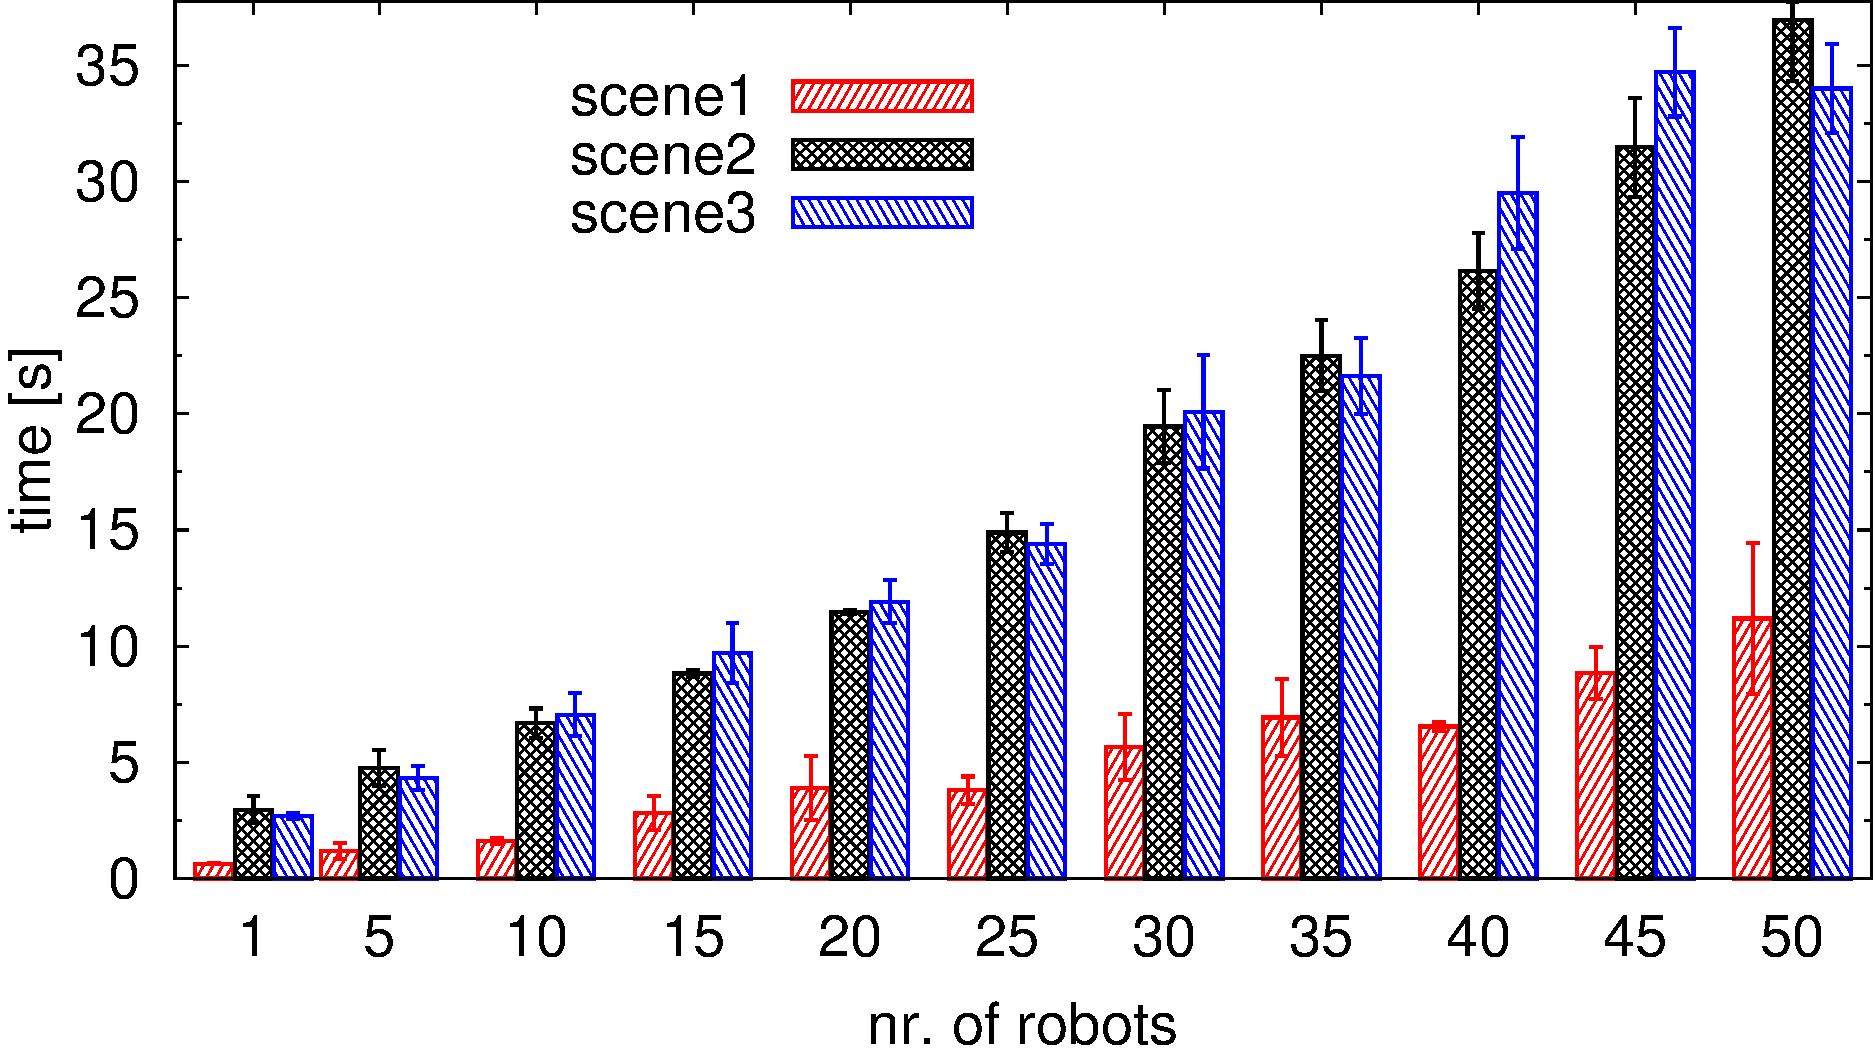
\includegraphics[width=0.85\textwidth]{figResT}
\caption{Results on the average time for all the boids to reach the
  final destination as a function of the number of boids. Bars
  indicate one standard deviation.}
\label{fig:ResT}
\end{figure}

\noindent
The efficiency of $\Name$ derives from the combination of global path
planning via probabilistic roadmaps with local path planning via
potential fields.  To test this further, we ran $\Name$ with 30 boids
but without the
probabilistic roadmap. In this scenario, the boids would be guided by
the potential fields and only be attracted to the final destination
but not to any intermediate goals. Without probabilistic roadmaps,
however, the approach timed out and failed to send any boid to the
final destination. These experiments indicate the importance of
combining probabilistic roadmaps with potential fields when planning
motions for large swarms in complicated environments.


Fig.~\ref{fig:ResFL} plots the average time difference between the
first and the last boid to reach the final destination. The plot
shows that the boids reach the final destination nearly at the same
time even as the number of boids is increased. These results indicate
that the boids remain together and move as a swarm.  

\begin{figure}
\centering
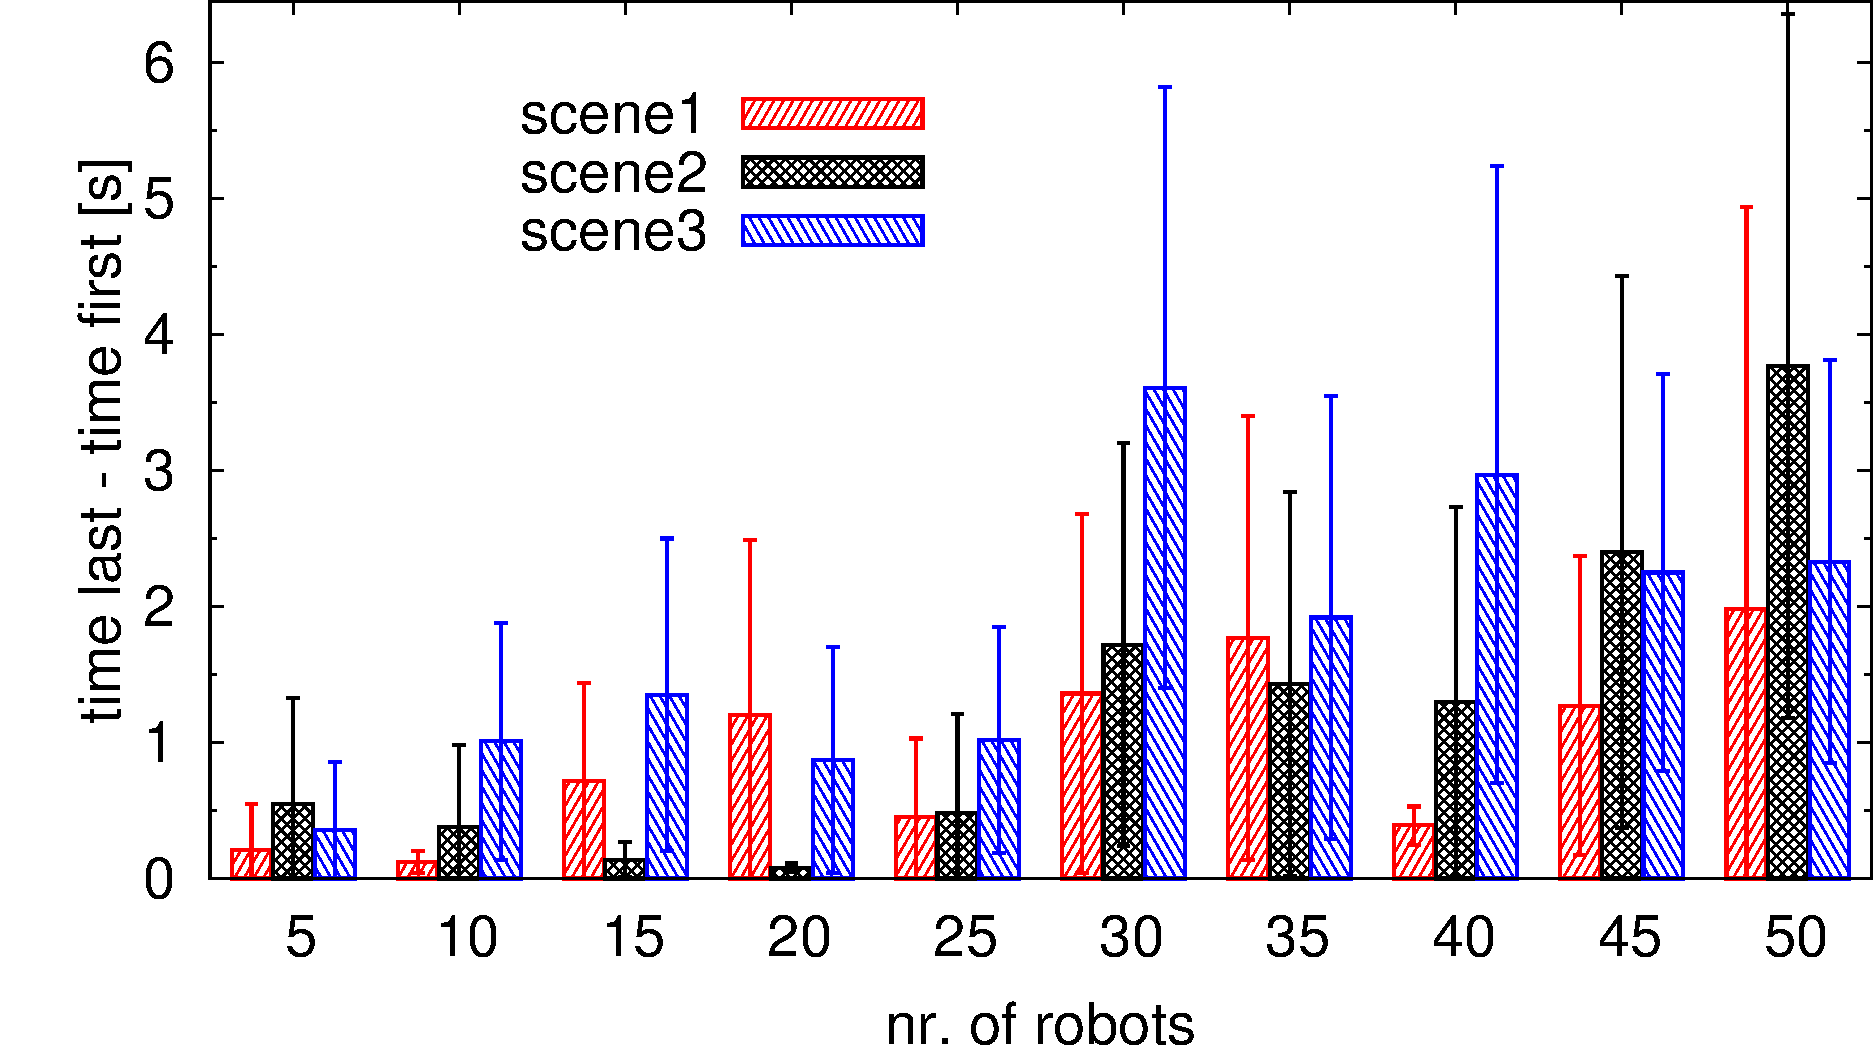
\includegraphics[width=0.85\textwidth]{figResFL}
\caption{Results on the average time difference between the first and
  the last boid to reach the
  final destination as a function of the number of boids. Bars
  indicate one standard deviation.}
\label{fig:ResFL}
\end{figure}

Fig.~\ref{fig:ResD} plots the average scaled distance among all boid
pairs (see Section~\ref{sec:Measures}). The scaled distance provides
an indication as to how close the boids are to one another. It is
desirable that the boids are neither too close (as it could cause
collisions or getting stuck in local minima) nor too far from each
other (as it could cause certain boids to get separated from the
swarm). The results indicate that the boids maintain a desirable
separation distance. Moreover, the separation distance changes very
little even as the number of boids is increased.


\begin{figure}
\centering
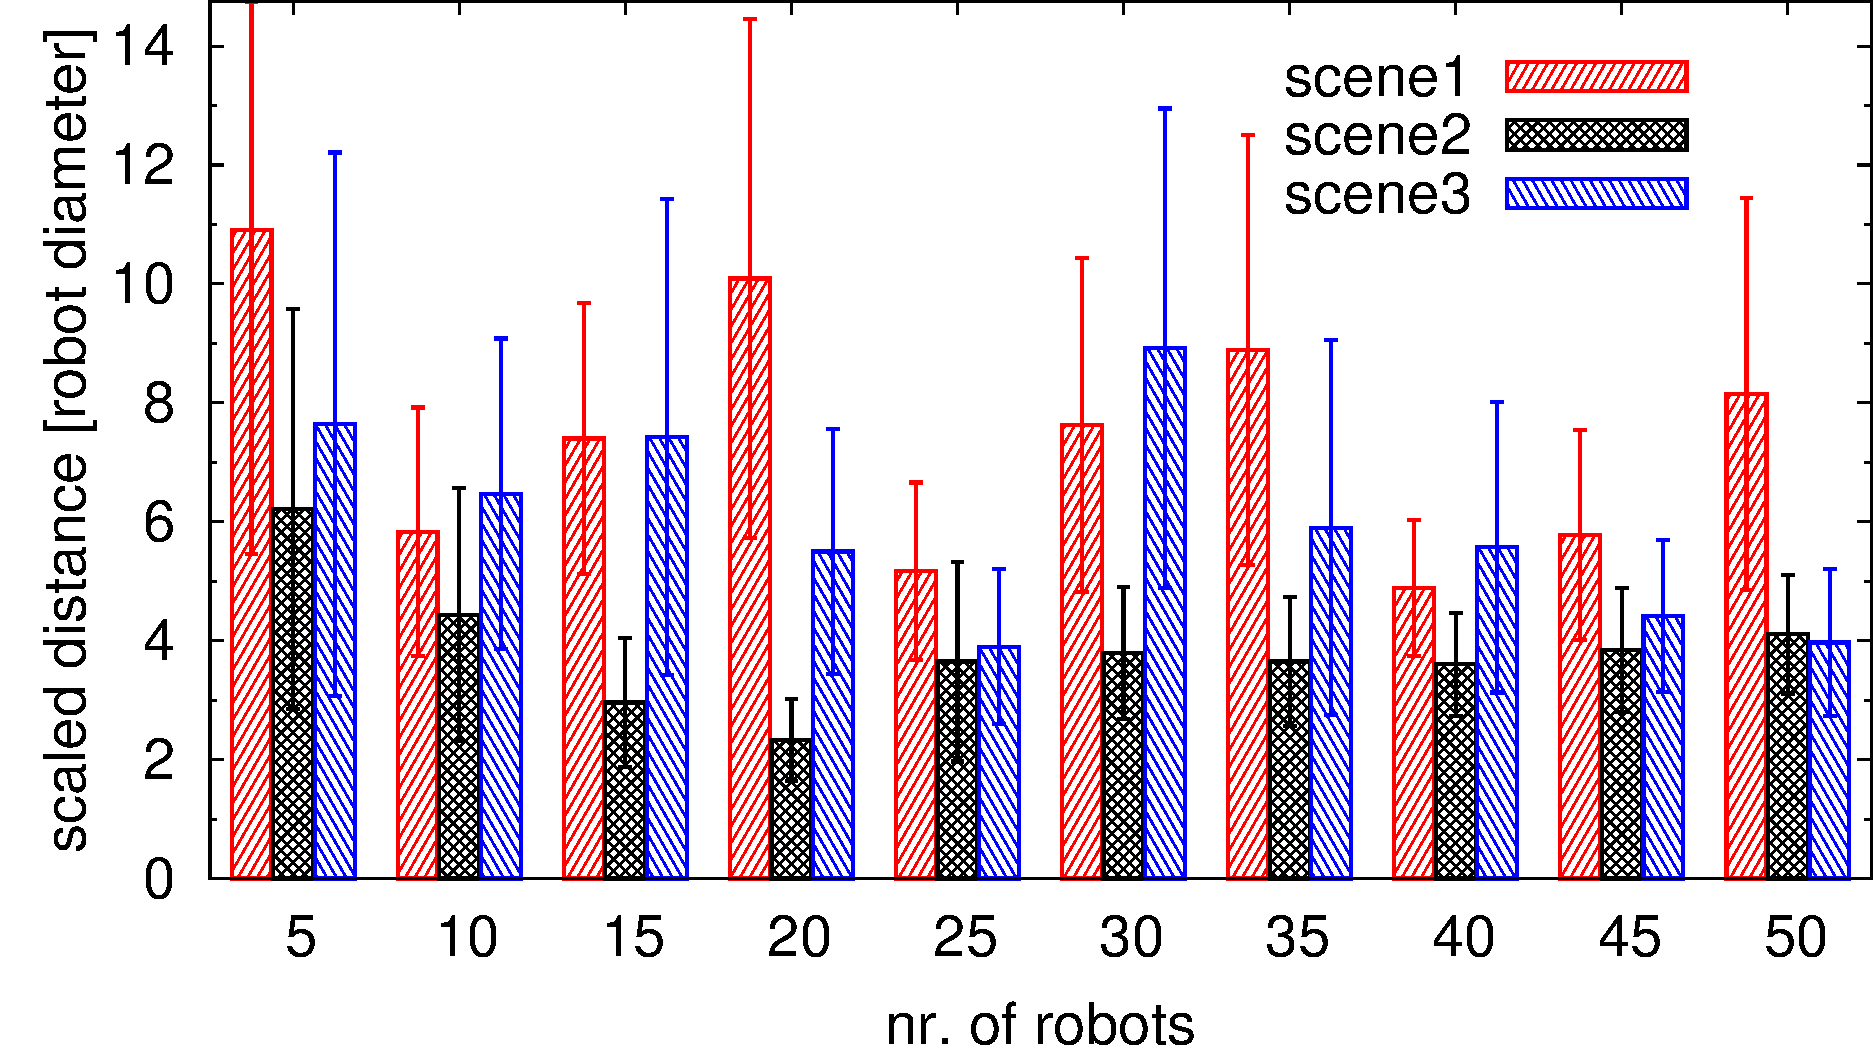
\includegraphics[width=0.85\textwidth]{figResD}
\caption{Results on the average scaled distance among all boid pairs
  as a function of the number of boids. Scaling is done with respect
  to the boid diameter. Bars
  indicate one standard deviation.}
\label{fig:ResD}
\end{figure}

\section{Discussion}

\bibliographystyle{splncs}
\bibliography{mp,plaku}
\end{document}

